\documentclass[letterpaper, 12pt]{article}
\usepackage{graphicx}
\usepackage{amsmath}

\graphicspath{{./pics/}}
\begin{document}
\title{6.013 Final project Report}
\author{Andres Erbsen, Justin Graves, Dimitris Koutentakis}
\date{\today}
\maketitle
\vspace{5mm}
\tableofcontents
\clearpage
\section{Introduction}
\section{Filter Design}
In order to design our filters, we had to apply some of the basic knowledge we acquired in the lectures towards the end of the semester. More specifically, we had to apply knowledge regarding transmission line resonators as well as smith charts and stubs.
\\
By calculating the dimensions for our given substrate and target frequencies we were able to build the filters desired. The filters that we ended up building are:
\begin{itemize}
    \item A short-short half wave resonator for $\lambda=?$,
    \item A short-short half wave resonator for $f=2.4 GHz$,
    \item A single stub band-stop resonator, and
    \item A multiple stub band pass approximation filter
\end{itemize}
\subsection{Short-short half wave resonator}
For the first short-short half-wave resonator, we used the dimensions of the original board given. More specifically, we used a length of $D=?$ and $\delta$ very small in order to maximize our $Q$. 
\begin{align*}
    D=
\end{align*}
\subsection{Short-short 2.4 GHz resonator}
In order to build a filter aimed at our radar's working frequency, we had to design and build a filter that would work at around 2.4 GHz. The calculations we made can be seen below:
\begin{equation*}
\left.
\begin{aligned}
    D&=\frac{m\cdot\lambda_n}{2} \\
    \lambda_n&=\frac{\lambda_0}{n}\\
    m&=1 \\
    \epsilon_r&=2.33 \\
    \mu_r&=1
\end{aligned}
\right \}
\Longrightarrow
D=0.0409m
\end{equation*}

\subsection{Single stub band-stop filter}
describe
\subsection{multiple stub band-pass filter}
describes
\section{Measurements}

\subsection{Short-short half wave resonator}
\begin{figure}
    \centering
    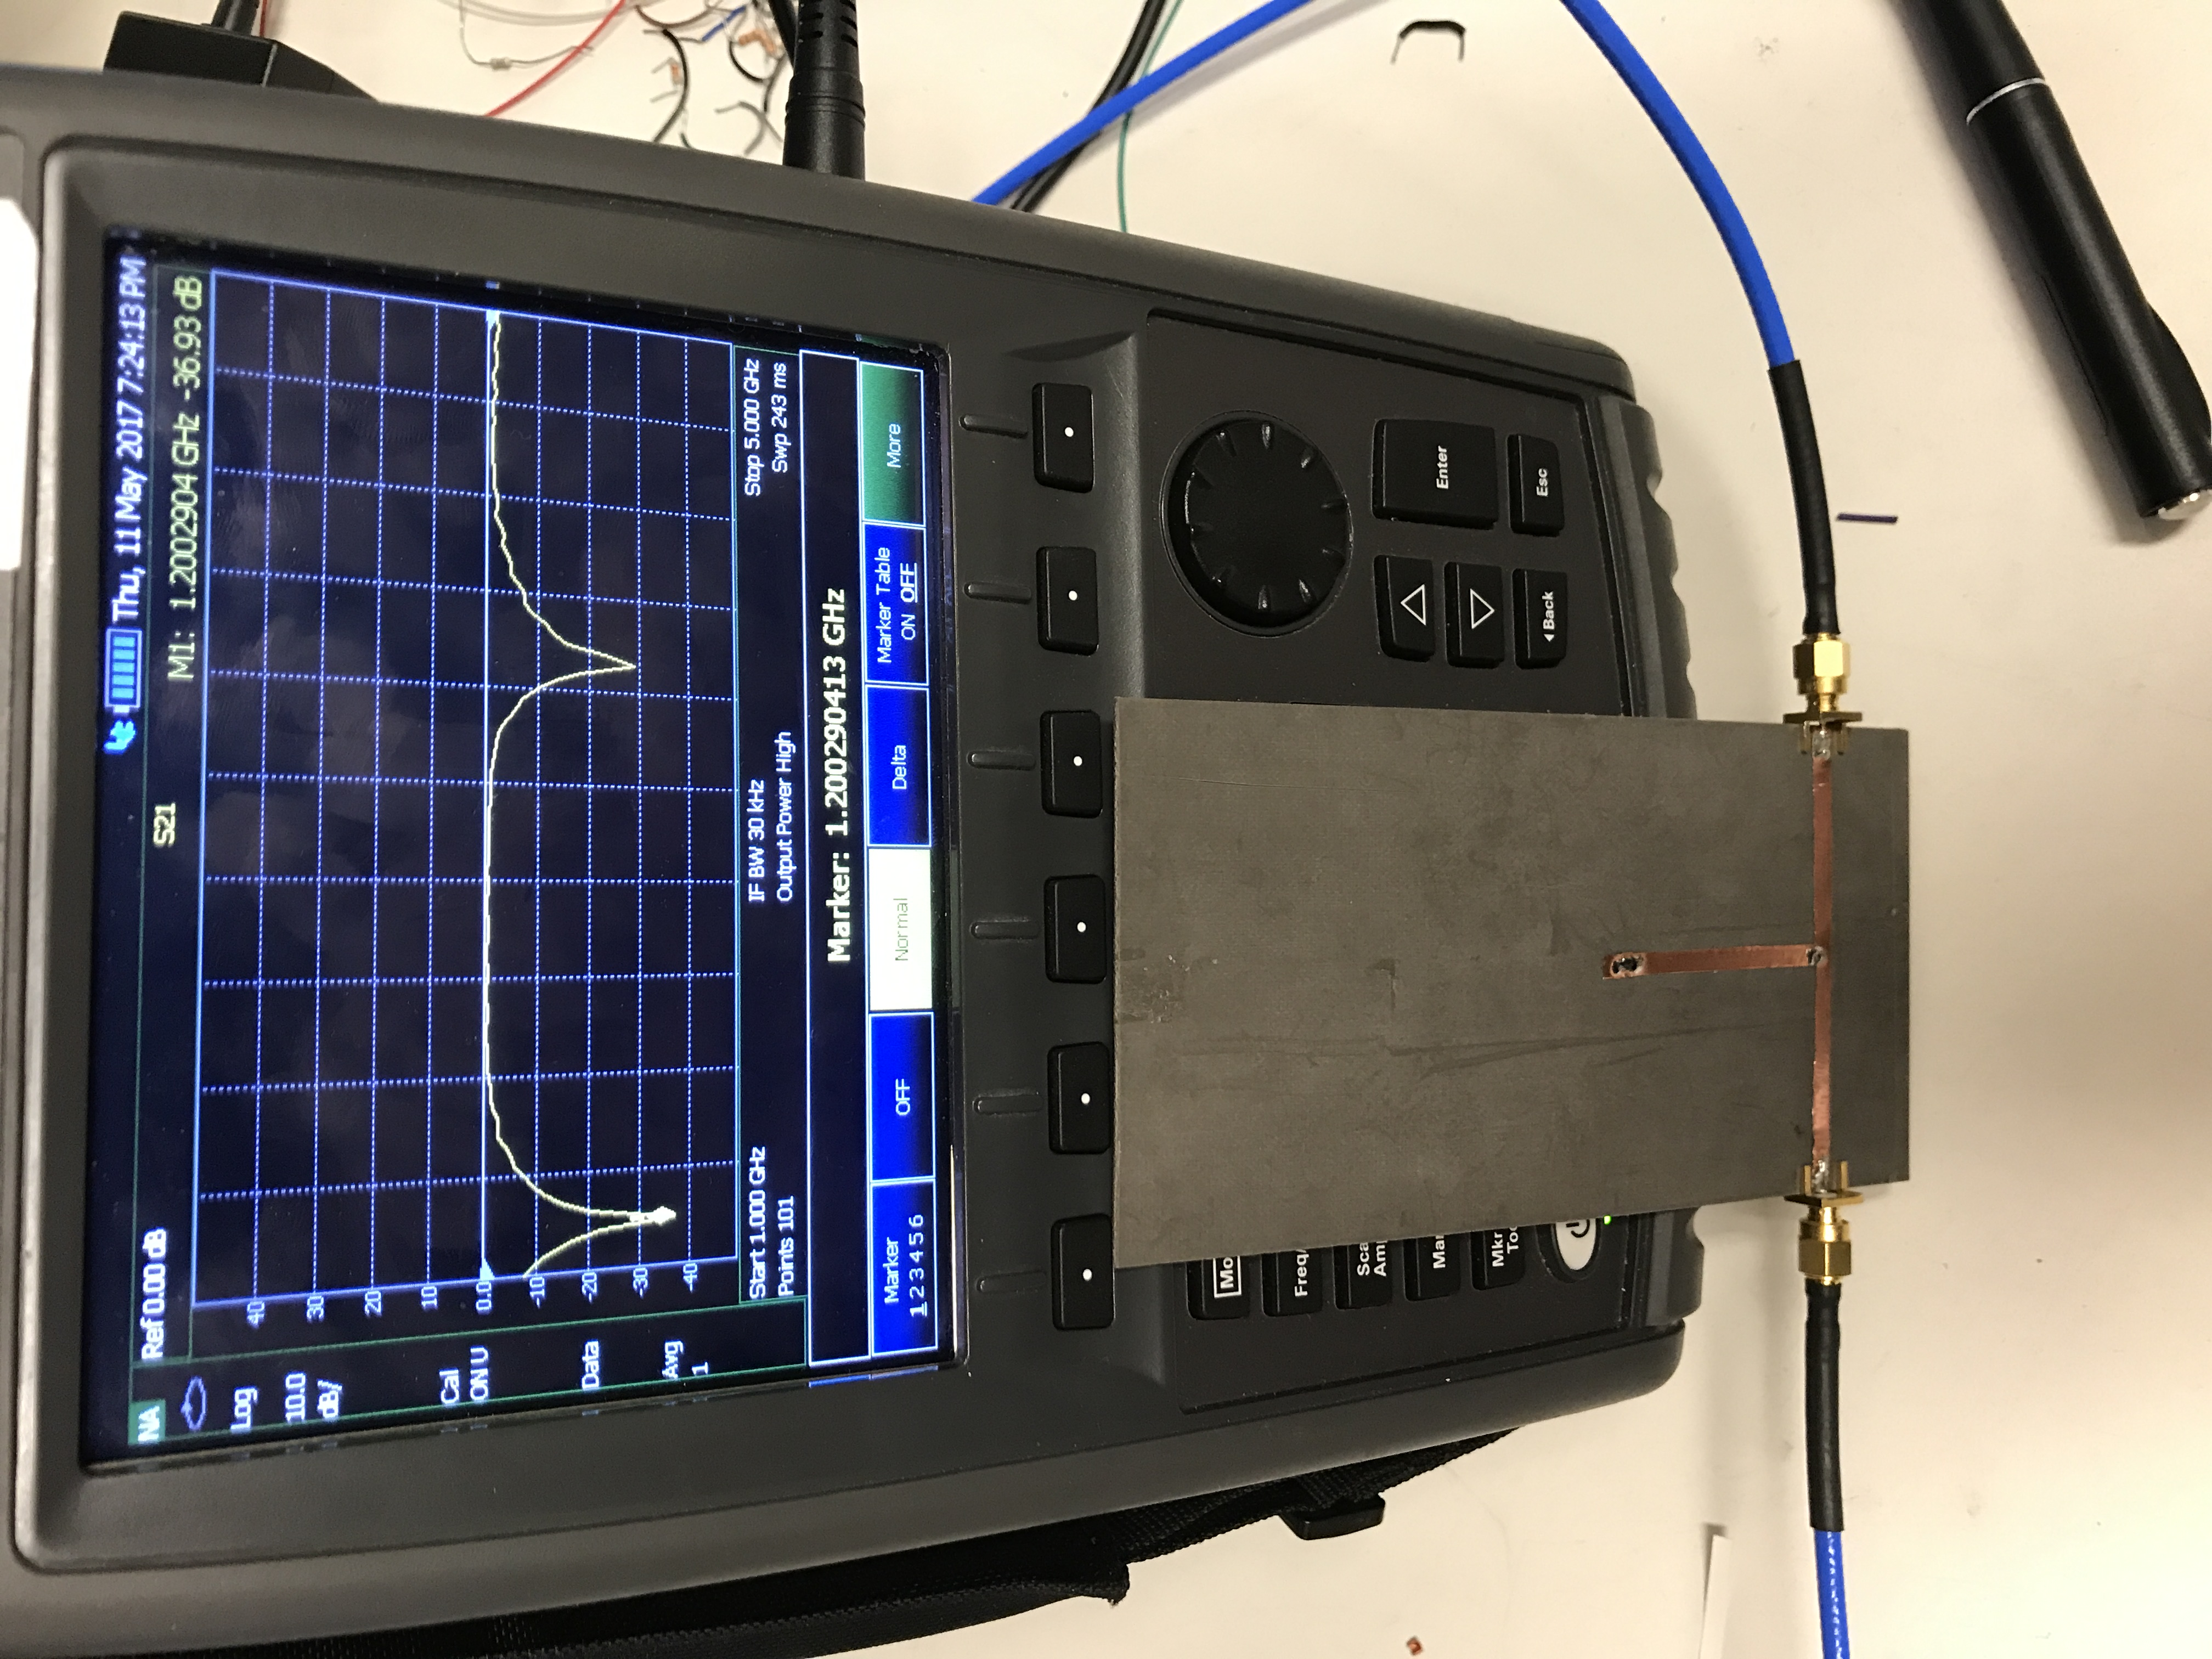
\includegraphics[width=0.8\textwidth, angle=270]{1stub}
    \caption {single stub measurements}
\end{figure}
\subsection{Short-short 2.4 GHz resonator}


\subsection{Single stub band-stop filter}
describe
\subsection{multiple stub band-pass filter}
describes

\section{Discussion}
describe
\end{document}

